


\chapter{Background}
\label{cha:background}

\section{Problem formulation}

We define a point cloud of the environment, $W$, as a set of points, $p \in W$, with the coordinates $[x, y, z] \in \mathbb{R}^{3}$. A robot is defined as a polygon, $R$. $W_{cov} \subset W$ is a set of points $p$ that are classified as coverable by the robot. A point, $p$, is coverable if $R$ can be placed in such way that no point in $W \textbackslash W_{cov}$ is inside $R$ if $p$ is inside $R$. Additionally, the height difference $|z_2 - z_1|$ between two points, $p_1$, $p_2 \in W_{cov}$, inside $R$ can not be bigger than the maximum robot step height, $h^R_{max}$.

The Coverage Path Planning (CPP) problem is to find a path $P$ with sequential positions $s \in P$ such that every point $p \in W_{cov}$ must have been inside $R$ at least once after placing $R$ at every position in $P$. $s$ is a 6D robot pose with a position $[x, y, z] \in \mathbb{R}^{3}$ and an orientation $[\phi, \theta, \psi]$ representing the yaw, pitch and roll.

\section{Properties}
There are unlimited ways to create a path that solves the CPP problem. The choice of plan has to be based on the most sufficient properties. These properties are described below.

\begin{itemize}
    \item \textbf{Coverage} - Coverage, $C$, is defined as
    \begin{equation}
        C =\frac{N^p_{cov}}{N^p_{tot}} 
    \end{equation}
    where $N^p_{cov}$ is the amount of covered points and $N^p_{tot}$ is the total amount of coverable points. In theory, $C$ has to be 1 to solve the CPP problem, but in reality it is often lower and balanced against other properties.
    \item \textbf{Length} - Efficiency is important to not waste time and energy. The length of the path is the total traveled distance when moving through all waypoints in a path. It should be as low as possible.
    \item \textbf{Rotation} - The optimal cleaning path for the sweeping robot is a straight path. Turns are not only expensive time wise and energy wise, but are also increasing the risk of missed spots. Therefore, a good path should have as few turns as possible. Comparisons are made either by counting the number of turns or by calculating the total amount of degrees that the robot rotated while executing the path. 
    \item \textbf{Computational time} - The complexity of CPP algorithms can vary a lot. Even though an algorithm with higher complexity gives a slightly better path, a lower complexity algorithm could be more attractive if it saves time and requires cheaper components. An algorithm with low computational time is also more applicable in bigger environments. 
    
    %\item \textbf{Memory usage} - Some algorithms requires a big amount of memory. By using algorithms with less memory consumption, cheaper components are required. Memory consumption can be calculated by memory usage profile programs \cite{resourcepkg}. 
\end{itemize}



\section{BA*}
\label{sec:BAstar}
BA* is an online CPP algorithm proposed in \cite{bastar}, that is based on Boustrephedon motions and the A* search algorithm. The algorithm consists of following steps.

\begin{enumerate}
    \item Cover the local area using the BM algorithm until a critical point is reached.
    \item Use a backtracking list to find the next starting point.
    \item Use A* to plan a collision free path to the next starting point.
    \item Shorten the path using the A*SPT algorithm.
    \item Follow the generated path and go to step 1 to cover a new area.
\end{enumerate}

The algorithm will keep repeating these steps until Step 2 can not find a new uncovered starting point.

\subsection{Step 1: BM algorithm}
The goal of the Boustrophedon motion, BM, algorithm is to cover an unknown area by moving one step at a time and create a two dimensional tiling model $M$ of the area. The tiles, $c$, are squares, with the size of the robot and are allowed overlap with each other. The steps can only be made in the north, south, west or east direction. The algorithm keeps exploring the area until the robot reaches a position where it can not move in any of these 4 directions, a critical point $c_{cp}$, see algorithm \ref{alg:BM}.

\begin{algorithm}[H]
\SetAlgoLined
\KwData{Starting point, $c_{sp}$. Model $M$ of the area.}
\KwResult{Updated model $M$ of the area. Critical point, $c_{cp}$. Path until critical point $P_{local}$.}
\textup{Set $CriticalPointFound \rightarrow false$} \\
$c_{curr}$ = $c_{sp}$ \\
$P_{local} = \emptyset$ \\ 
\While{\textup{$CriticalPointFound$ is $false$}}{
    \textup{Set $CriticalPointFound \rightarrow true$} \\
    \For{\textup{position} $c_n$ \textup{in direction $n \in$ north, south, east, west from $c_{curr}$}}{
        \If{\textup{$c_n$ is available}}{
            \textup{Add tile $c_n$ to $M$} \\
            \textup{Add tile $c_n$ to $P_{local}$} \\
            $c_{curr}$ = $c_{n}$ \\
            \textup{Set $CriticalPointFound \rightarrow false$} \\
            \textbf{\textup{break}} \\
        }
    }
}
$c_{cp}$ = $c_{curr}$ \\
\textup{\textbf{return}} M, $c_{cp}$, $P_{local}$

 \caption{BM algorithm}
 \label{alg:BM}
\end{algorithm}

\subsection{Step 2: Find next starting point}
After a critical point has been reached, the algorithm has to find a new starting point for exploring the next area. This is made by adding specific tiles to a backtracking list while covering areas (Step 1). The backtracking list, $L_b$, is defined as
\begin{equation}
    L_b = \{ c | c \in M  \textup{ and } \mu(c) \ge 1  \},
\end{equation}

where $\mu(c)$ is 
\begin{equation}
    \mu(c) = b(c_1,c_8) + b(c_1,c_2) + b(c_5,c_6) + b(c_5,c_4) +b(c_7,c_6) + b(c_7,c_8) ,
\end{equation}
and $b(c_i, c_j)$ is

\begin{equation}
    b(c_i, c_j) = \begin{cases} 
        1, & \mbox{if } c_i \mbox{ is free and } c_j \mbox{ is blocked}\\ 
        0, & \mbox{otherwise} 
    \end{cases}.
\end{equation}

$c_i$ is a neighbouring cell to $c$ according to figure \ref{fig:tilesdefinition}. A cell is blocked if it has been visited or if it is inaccessible by the robot.

\begin{figure}
    \centering
    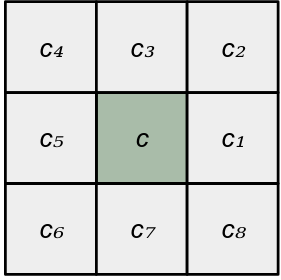
\includegraphics[width=0.3\textwidth]{figures/tilesscheme.png}
    \caption{Definition of a neighbouring cell $c_i$ of $c$. Used in BA* to find the next starting point.}
    \label{fig:tilesdefinition}
\end{figure}

The next starting point, $c_{sp}$ is chosen by picking the position of the closest cell $c \in L_b$ according to Euclidean distance, Manhattan distance or shortest path using only covered cells.

\subsection{Step 3: A* algorithm}
A* algorithm is a well known search algorithm that can be used to find the optimal path between two points in a grid or graph. The idea is to use a heuristic estimate,
\begin{equation}
    \label{eq:heuristic}
    f(s) = g(s) + h(s),
\end{equation}
where $g(s)$ is the length of the shortest path from the starting position, $s_{s}$ to $s$ that has been found so far and $h(s)$ is the estimated length between $s$ and the goal $s_g$. The algorithm is described in algorithm \ref{alg:astar}. It uses a priority queue, $Q_{open}$, which stores points that has been found, but it's neighbours has not been evaluated yet. The priority is based on $f(s)$ in equation \ref{eq:heuristic}. It means that the $\texttt{pop}$ function always returns the point with the smallest $f(s)$ and removes it from the priority queue. Every iteration starts with applying $\texttt{pop}$ on $Q_{open}$. The returned point is then moved to a list, $Q_{closed}$, to keep track of the points that have been visited. Thereafter, the neighbours of this point are evaluated to see if the estimated length of the total path gets shorter if the path goes through them. If that is the case or if a neighbour has not been visited, it gets a new $g(s)$ value and is added to the $Q_{open}$ list. It also gets the original point as $parent$. The $parent$ property is used at the end to backtrack the path when the goal point has been reached.

In BA*, this algorithm is used to find the shortest path from the critical point $c_{cp}$ (from Step 1) to the next starting point $c_{sp}$ (from Step 2).

\begin{algorithm}[H]
\SetAlgoLined
\KwData{Starting point, $s_{s}$. Goal point, $s_{g}$}
\KwResult{Path from  $s_{s}$ to $s_{g}$, $P$}
$Q_{open}$ =\textup{empty priority queue} \\
$Q_{closed} = \emptyset$ \\
$g[s_{s}]$ = 0 \\
$parent[s_{s}] = s_{s} $\\
$Q_{open}$.\texttt{push}($s_{s}$, $g[s_{s}] + \texttt{heuristic}(s_{s})$)\\
\While{\textup{$Q_{open}$ \neq \emptyset}}{
    $s \leftarrow Q_{open}.\texttt{pop}()$\\
    \If{\textup{$s$ is $s_{g}$}}{
        $P = \emptyset$ \\
        \While{\textup{$s$ is not $s_{s}$}}{
            $P.\texttt{push\_back}(s)$ \\
            $s \leftarrow parent[s]$
        }
        \textbf{\textup{return}} \textup{reversed $P$}
    }
    $Q_{closed}.\texttt{push}(s)$ \\
    \For{ \textup{neighbour $s_n$ of $s$}}{
        \If{\textup{$s_n$ not in $Q_{closed}$}}{
            \If{\textup{$s_n$ not in $Q_{open}$ or $g[s]$ + \textup{Distance between $s$ and $s_n$} < $g[s_n]$ }}{
                $g[s_n]$ = $g[s]$ + \textup{Distance between $s$ and $s_n$} \\
                $parent[s_n]$ = s \\
                $f$ =  $g[s_n]$ + $\texttt{heuristic}(s_n)$\\
                \eIf{ $s_n \in Q_{open}$ }{
                    $Q_{open}[s_n] = f$ \\
                }{
                    $Q_{open}.\texttt{push}(s_n, f) $
                } 
            }
        }
    }
}
\caption{\textup{A* algorithm}}
\label{alg:astar}
\end{algorithm}

\subsection{Step 4: A*SPT Algorithm}
The A* algorithm in Step 3 generates a collision free path, $P$, from the critical point $c_{cp}$ to the next starting point $c_{sp}$. Since this path is based on square tiles, it often includes a lot of heading changes. Consequently, it will not be the shortest path. A*SPT is an algorithm that takes a path as input and smooths it out to make it shorter and unbounded to the tile model, see algorithm \ref{alg:astarSPT}. The idea is to find the farthest point from the start with a line-of-sight and add it to the smooth path $\hat{P}$. This is repeated until the found point is the goal point.

\begin{algorithm}[H]
\SetAlgoLined
\KwData{Path $P$ = $\{s_1, s_2, ..., s_n\}$}
\KwResult{Smooth path $\hat{P}$ = $\{\hat{s}_1, \hat{s}_2, ..., \hat{s}_k\}$}
$k =1$ \\
$\hat{P} = \{s_{1}\}$\\
\While{\textup{$s_k$ is not $s_n$}}{
    \For{ i \in $n$, $ n-1$, ..., $ k+1$ }{
        $P_{s_k, s_i}$ = \textup{Straight line path between $s_k$ and $s_i$}\\
        \If{\textup{$P_{s_k, s_i}$ is collision free}}{
            $\hat{P}.\texttt{push\_back}$($s_i$)\\
            \textup{Set $k \rightarrow k + 1$} \\
        }
    }
}
\textup{\textbf{return} $\hat{P}$}

 \caption{A*SPT algorithm}
 \label{alg:astarSPT}
\end{algorithm}

\subsection{Step 5: Follow path and go back to Step 1}
When the smooth path $\hat{P}$ between the critical point and the next starting point has been generated, the next step is to make the robot follow this path. When the next starting point is reached, the algorithms goes back to Step 1 and repeats the process.

% this path by adjusting the heading angle and move the distance between the points. Assuming that the robot is currently at tile $c_i$ at position $(x_i, y_i)$ and has the heading angle $\theta$, the robot needs to turn 
% \begin{equation}
%     \alpha = \arctan{\frac{y_{i+1} - y_i}{x_{i+1} - x_i}} - \theta
% \end{equation}

% and move the distance
% \begin{equation}
%     d = \sqrt{ (y_{i+1} - y_i)^2 + (x_{i+1} - x_i)^2 }
% \end{equation}
% to get to the next starting point. Before exploring the new area it has to turn towards a available neighbour tile in the priority order north-south-east-west. The angle of the turn will be
% \begin{equation}
%     \beta = \gamma - \alpha, \beta \in (-\pi, \pi]
% \end{equation}
% where $\gamma$ equals to $\pi/2, -\pi/2$, 0  or $\pi$ if the neighbour is in the direction north, south, east or west respectively. 

\section{Inward Spiral}
 \label{sec:spiral}
The Inward Spiral is a grid-based solution to the coverage path planning problem proposed in \cite{inwardsspiral}. The idea is to clean the area counter-clockwise (or opposite) by keeping the robot as much to the right as possible and only turn left if the grid cell in front of the robot has been cleaned already or is untraversable. This continues until the robot has no options, reaches a dead zone. By using a wavefront algorithm, it then finds the closest grid cell that has not been cleaned and finds the shortest path to that point using A*. This cycle repeats until the area has been covered. In summary:

\begin{enumerate}
    \item Clean area in an inward spiral motion until a dead zone is reached
    \item Find closest uncovered accessible cell using Wavefront algorithm.
    \item Find shortest path using A* to the closest uncovered cell and go back to Step 1.
\end{enumerate}

\subsection{Step 1 - Clean area in an Inward spiral motion}

The inward spiral motion starts in a corner of the area. If the counter-clockwise the direction is chosen it then follows the right wall until it reaches an obstacle or a covered cell. The algorithm to create this movement is described in Algorithm \ref{alg:inwardspiral}.

\begin{algorithm}[H]
\SetAlgoLined
\KwData{Current position, $c_{curr}$}
\KwResult{Path until dead zone, $P$}
\textup{Set $DeadZoneReached \rightarrow false$} \\
$P$ = $\{c_{curr}\}$ \\
\While{\textup{$DeadZoneReached$ is $false$}}{
    \textup{Set $DeadZoneReached \rightarrow true$} \\
    \For{\textup{neighbour $c_n$ of $c_{curr}$ for $n \in $  right, forward, left }}{
        \If{\textup{$c_n$ is covered or inaccessible}}{
            \textup{\textbf{continue}}\\
        }
        $P.\texttt{push\_back}$($c_n$) \\
        \textup{Set $c_{curr} \rightarrow c_n$} \\
        \textup{Set $DeadZoneReached \rightarrow false$} \\
        \textup{\textbf{break}}\\
    }
}
\textup{\textbf{return}} $P$

 \caption{Generate path that cover the area in an inward spiral motion until a dead zone has been reached}
 \label{alg:inwardspiral}
\end{algorithm}

\subsection{Step 2 - Find closest uncovered cell using Wavefront algorithm}

After reaching a dead zone the robot needs a new starting point for the next inward spiral motion. Since this method is grid based a Wavefront algorithm can be used to find the closest uncovered cell that is free from obstacles. The idea is to walk layer by layer, $L_k$, from the original robot position $c_s$ to find the closest uncovered obstacle free cell, see details in Algorithm \ref{alg:wavefront} and figure \ref{fig:wavefront}.

\begin{figure}
    \centering
    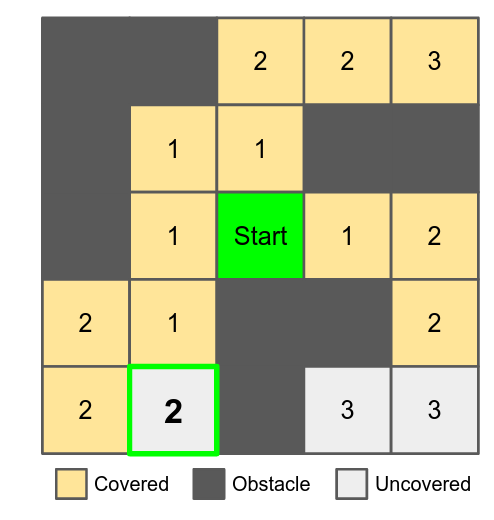
\includegraphics[width=0.5\textwidth]{figures/wavefront.png}
    \caption{An example of the wavefront algorithm. The number in the cells represents the number of steps from START. The goal of the algorithm is to find the closest uncoverable cell.}
    \label{fig:wavefront}
\end{figure}

\begin{algorithm}[H]
\SetAlgoLined
\KwData{Start cell, $c_s$}
\KwResult{Closest uncovered obstacle free cell $c_f$}
$k=0$ \\
$L_{0} = \{c_s\}$ \\
$V = \{c_s\}$\\
\While{\textup{$L_{k}$ \neq \emptyset}}{
    $L_{k+1}$ = \emptyset \\
    \For{ \textup{cell $c \in L_{k}$} }{
        \For{ \textup{neighbour $c_n$ of $c$} }{
            \If{\textup{$c_n$ is not obstacle free or is in $V$}}{
                \textup{\textbf{continue}} \\
            }
            \If{\textup{$c_n$ is uncovered}}{
                \textup{\textbf{return} $c_n$} \\
            }
            $V = V \cup c_n$ \\
            $L_{k+1} = L_{k+1} \cup c_n$ \\
        }
    }
    \textup{Set $k \rightarrow k+1$} \\

}

\textup{\textbf{return}} $Failure$

 \caption{Wavefront algorithm. Finds the closest uncovered obstacle free cell.}
 \label{alg:wavefront}
\end{algorithm}

If the algorithm does not find a new starting point, the area has been fully covered and the path planning is finished.

\subsection{Step 3 - Find shortest path using A* to the closest uncovered cell}

When a new starting point has been discovered, the shortest path from the current robot position to the new starting point is generated using A*, which is described in detail in Algorithm \ref{alg:astar}. After reaching the point, the algorithm goes back to step 1 and covers the area in an inward spiral motion until a new dead zone is reached. 

\section{Sampling-Based Coverage Path Planning}
\label{sec:randomsample}
An approach that could be used to cover 3D structures was proposed by B. Englot and F. Hover in \cite{6386126}. The approach can be divided into following steps:

\begin{enumerate}
    \item Locate planar areas and waypoints for simple zig-zag covering.
    \item Find waypoints in individual complex areas with randomized sampling.
    \item Remove redundant waypoints using greedy and pruning algorithms.
    \item Create a sequence of points that visits all waypoints using the Traveling Salesman Problem algorithm Lin-Kernighan.
    \item Create collision free paths between all waypoints using RRT.
\end{enumerate}

Since the main application of this apporach is autonomous underwater exploration of a ship hull, some details can be simplified for the sweeping robot case.  

\subsection{Step 1 - Planar areas}
The first step is to segmentize the data representing the environment into planar areas. In \cite{6386126}, this was made with a method proposed in \cite{segmentiseplanar} where the data was a triangle mesh.

The next step is to generate waypoints for every plane. This is done by choosing a random point on the plane and expand a grid of waypoints in the four directions north, south, east and west. It generates new waypoints in every direction along the plane until collision or if the waypoint is out of range to cover the plane. This generates a set of paths that covers all planar areas in the environment.

%see algorithm \ref{alg:planewaypoints}. At first, a random point, $p_i$ on the plane is chosen. Secondly a random point $q$ is sampled such that $p_i$ lies within the range of the sensor assuming that the underwater vehicle is placed at $q$. A new plane, $SweepPlane$, which is parallel with the original plane, $P_k$, is then generated based on the height of $q$ and the normal of $P_k$. A waypoint grid, $Q_k$, is then expanded from $q$ along $SweepPlane$ in all four north-south-east-west directions until collision or if the point is out of range to cover $P_k$. The yaw angle of the north direction is selected by evaluating the covariance matrix of the plane and make the grid fit the plane as good as possible.

% \begin{algorithm}[H]
% \SetAlgoLined
% \KwData{Segmented planes $S$, robot range $r$}
% \KwResult{Set of waypoints that covers plane areas $Q$}

% \For { \textup{plane $P_k$ \in $ S$} }{
%     $p_i$ = \textup{random point in plane $P_k$} \\
%     \While{\textup{$q$ is not collision free point}}{
%         $q$ = \textup{random point within distance $r$ from $p_i$}\\
%     }
%     Q_k \leftarrow q\\
%     $ExpansionComplete = false$\\
%     $SweepPlane$ = \textup{A plane parallel to $P_k$ including $q$}\\
%     \While { \textup{not $ExpansionComplete$}}{
%         \For {\textup{direction, $d \in $ \{ north, east, south, west \}}}{
%             Q_k^{d} = \textup{Expand $Q_k$ in direction $d$ along $SweepPlane$} \\
%             Q_k = Q_k \cup Q_k^{d}\\
%         }
%         \If{$Q_k^{north} \cup Q_k^{east} \cup Q_k^{south} \cup Q_k^{west} = \emptyset$}{
%             ExpansionComplete = true\\
%         }
%     }
%     Q \leftarrow Q_k\\
% }
% \textup{\textbf{return}} $Q$

%  \caption{Generate waypoints that cover planar areas}
%  \label{alg:planewaypoints}
% \end{algorithm}

\subsection{Step 2 - Complex areas}

Waypoints on complex areas that could not be expressed as planes are generated using random sampling. The algorithm samples positions until every coverable point could be covered from $k$ different sampled positions. 

%, see algorithm \ref{alg:complexwaypoints}. This algorithm sample waypoints until every point is covered by at least $k$ waypoints,  

% \begin{algorithm}[H]
% \SetAlgoLined
% \KwData{Points in complex areas $P$, robot range $r$, number of times to cover each point $k$}
% \KwResult{Set of waypoints that covers complex areas $Q$}

% $KCoverageComplete = false$\\
% $Q$ = \emptyset \\
% \While{\textup{not $KCoverageComplete$}}{
%     $p_i$ = \textup{point in $P$, which is not within a range of $k$ points in $Q$} \\
%     \While{\textup{$q$ is not a collision free point}}{
%         $q$ = \textup{random point within distance $r$ from $p_i$}\\
%     }
%     $Q$ \leftarrow $q$ \\
%     \If {\textup{each point in $P$ is within a range of $k$ points in $Q$}}{
%         $KCoverageComplete = true$ \\
%     }
% }
% \textup{\textbf{return}} $Q$

%  \caption{Generate waypoints that cover complex areas}
%  \label{alg:complexwaypoints}
% \end{algorithm}

\subsection{Step 3 - Remove redundant waypoints}
After Step 1 and 2 each point in the area should be covered at least once if the robot visits all the waypoints. Since some points are covered more than once, there is a possibility that some of them could be removed, which would reduce the computational time and memory usage of the algorithm in the following steps. The following algorithms were proposed in \cite{JOHNSON1974256}, and applied in \cite{6386126}.

At first, a greedy algorithm will be used. It iteratively chooses the set, the path for planar areas and the waypoint for complex areas, that covers most uncovered points until all points have been covered at least once. 

Then, a pruning algorithm removes every set that does not cover a point uniquely. It iteratively chooses the set that minimizes the overlapping with covered points. This algorithm is also applied to individual rows and columns of the path grids that covers the planar areas.

% \begin{algorithm}[H]
% \SetAlgoLined
% \KwData{Plane areas with waypoints $Q_{planes}$, Waypoints on complex areas $Q_{complex}$ }
% \KwResult{Minimal amount of waypoints that covers the area, $Q_{sub}$}

% $SUB_1$ = \emptyset \\
% $SETS$ = $Q_{complex} \cup Q_{planes}$ \\
% $UNCOV_1$ =  $SETS$ \\
% \While{ $UNCOV_1  \neq \emptyset$ }{
%     S_j = Max( |S| \textup{ for $S$ in } SETS )\\
%     $SUB_1$ \leftarrow S_j \\
%     $UNCOV_1$ = $UNCOV_1 \backslash S_j$ \\
%     \For{$S \in SETS$}{
%         $S = S \backslash S_j$ \\
%     }
% }

% \For{S \in SUB_1}{
%     \If {$S_j \in Q_{planes}$}{
%         $Q_{rowcol}$ = \textup{Rows and columns of grid $S_j$ as sets}\\
%         SUB_1 \leftarrow Q_{rowcol}\\
%         $SUB_1$ = $SUB_1 \backslash S_j$ \\
%     }
% }

% $Q_sub$ = \emptyset \\
% $UNCOV_2$ =  $SUB_1$ \\
% $LEFT$ =  $SUB_1$ \\
% \While{ $UNCOV_2 \neq \emptyset$ }{
%     S_j = Min( |S - UNCOV_2| / |S \cap UNCOV_2| \textup{ for $S$ in } LEFT )\\
%     $Q_sub$ \leftarrow S_j \\
%     $UNCOV_2$ = $UNCOV_2 \backslash S_j$ \\
%     \For{$S \in LEFT$}{
%         $S = S \backslash S_j$\\
%     }
% }
% \textup{\textbf{return}} $Q_sub$


%  \caption{Greedy and pruning algorithm to remove redundant waypoints.}
%  \label{alg:greedypruning}
% \end{algorithm}


\subsection{Step 4 - Traveling Salesman}
When the minimum amount of waypoints to cover the area has been generated, the next step is to generate the path, that visits all waypoints. Before solving this problem, which is called Traveling Salesman Problem (TSP), all waypoints has to be represented as a graph.

The path through the grids on planar areas is trivial since it is a basic zig-zag motion. Therefore, each planar area path can be reduced to a pair of points to represent the entry and exit. To ensure that this pair appear adjacent in the TSP solution, the cost of the edge between them, is set to zero. All other edges between nodes are given a cost of the Euclidean distance plus a large number big enough to ensure that the entry-exit pair will be adjacent in the TSP solution.

There are many ways to solve the TSP. One of the most effective way, which was used in \cite{6386126}, is to use Lin-Kernighan algorithm \cite{Helsgaun00aneffective}. It is an approximate algorithm giving a non-optimal solution in a relatively short time. The idea is to start with a tour that is generated in a randomized way and improve it until no more improvements are possible. 

%This is made by at each iteration find two sets of links between waypoints such that, if the first one would be replaced by the second, it would result in a shorter tour. A big advantage of the Lin-Kernighan algorithm comparing to other similar algorithms is that the size of these sets are variable. It makes it more flexible and efficient for different applications since it is difficult to find the best compromise between path length and computational time in advance. 

The entry and exit of the sweep paths were defined before starting the TSP algorithm. Since it is possible that another order or set of entries and exits gives a better solution, different combinations are tested to see if any changes results in a shorter path.

\subsection{Step 5 - RRT}

After generating a sequence of waypoints, a bi-directional rapidly-exploring random tree (RRT) algorithm is used to find collision free paths between the waypoints. RRT, described in algorithm \ref{alg:RRT}, builds two search trees, that are biased to grow towards each other. When the two trees meet, a path that goes from starting point $p_s$ to goal point $p_g$ is generated. The trees grow using the function $\texttt{extend}$, see algorithm \ref{alg:extend}. At first, one of the trees is extended towards a random sampled point $p_{rand}$. If the extension was successful and generated a new point $p_{new}$, the other tree is extended towards $p_{new}$. Before the next iteration, the trees get swapped, meaning that the second tree will now be extended towards a new random sampled point. \cite{rrt}

The first step of the $\texttt{extend}$ function is to find the point, $p_{near}$, in the search tree, $T$, that is the closest to the given point, $p_{ext}$. The second step is to generate a point, $p_{new}$, at a user defined distance from $p_{near}$ towards $p_{ext}$. If $p_{new}$ is a traversable point, the point and the edge from $p_{near}$ to $p_{new}$ is added to the search tree.  This is illustrated in figure \ref{fig:extend}. The status of the point is set to $Reached$ if the point reached $p_{ext}$, $Trapped$ if it was untraversable and $Advanced$ if it was traversable, but did not reach $p_{ext}$. \cite{rrt}

\begin{figure}
    \centering
    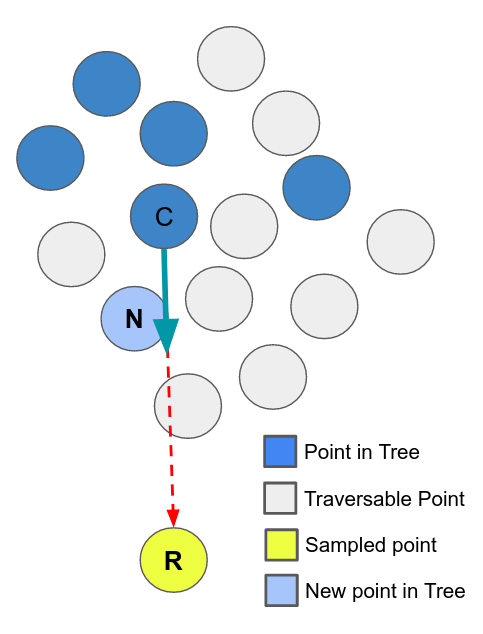
\includegraphics[width=0.4\textwidth]{figures/extend.png}
    \caption{Illustration of the $\texttt{extend}$ algorithm. $R$ represents the sampled $p_{ext}$ point, $C$ is the closest point in the tree $p_{near}$ and $N$ is the new node in the tree $p_{new}$.}
    \label{fig:extend}
\end{figure}

\begin{algorithm}[H]
\SetAlgoLined
\KwData{Search tree $T$, point defining the direction of extension $p_{ext}$, step size $\lambda_{RRT}$}
\KwResult{New point $p_{new}$}

\textup{$p_{near} =$ closest point in $T$ from $p_{ext}$}\\ 
\textup{$p_{new} =$ point not in $T$ closest to the position that is at a distance $\lambda_{RRT}$ towards $p_{ext}$ from $p_{near}$}\\ 
\eIf{\textup{$p_{new}$ is traversable}}{
    T = T \cup \{p_{new\}}\\
    \eIf{\textup{$p_{new}$ is $p_{ext}$}}{
        $status[p_{new}] = Reached$\\
    }{
        $status[p_{new}] = Advanced$\\
    }
}{
    $status[p_{new}] = Trapped$\\
}
\textup{\textbf{return} $p_{new}$}\\

 \caption{Extend algorithm}
 \label{alg:extend}
\end{algorithm}

\begin{algorithm}[H]
\SetAlgoLined
\KwData{Point cloud of environment $W$, Start point, $p_s$, Goal point, $p_g$, Max iterations $N^{RRT}_{max}$}
\KwResult{Path $P$ from $p_s$ to $p_g$ }

T_a = \{p_s\} \\
T_b = \{p_g\}  \\
\For{$k \in 1, 2, ..., N^{RRT}_{max}$}{
    \textup{$p_{rand}$ = random sampled point in $W$}\\
    p_{new} = \texttt{extend}(T_a, p_{rand})\\
    \If{$status(p_{new}) \neq Trapped$}{
        \If{\textup{$status(\texttt{extend}(T_b, p_{new}))$ is $Reached$}}{
            \textup{\textbf{return} Shortest path from $p_s$ to $p_g$ through $T_a$ and $T_b$}\\
        }
    }
    \texttt{swap}(T_a, T_b)\\
}
\textup{\textbf{return} $Failure$}

 \caption{RRT Path Planning Algorithm to find a path between to points.}
 \label{alg:RRT}
\end{algorithm}

When collision free paths between the points have been generated, the cost of the edges between the waypoints are set to the distance of the generated paths. Finally, the TSP algorithm is repeated with the updated costs until a stable solution is found.

